\chapter{Transforming Functions}
Recall how we could translate, mirror, or rotate shapes and they would still be congruent shapes? We can do the same with functions, but the functions are not always equal.
Let's say we gave you the graph of a function $f$, like this:
\begin{figure}[htbp]
    \centering
        \begin{tikzpicture}
            \begin{axis}[
                xmin=-2.2,xmax=2.2,
                ymin=-1,ymax=5,
                axis x line=middle,
                axis y line=middle,
                axis line style=<->,
                xlabel={$x$},
                ylabel={$y$},
            ]
            \addplot[no marks,sdkblue] expression[domain=-2:2,samples=100]{x^2} node[below, yshift=-6mm] {$f(x)$};
            \end{axis}\end{tikzpicture}
    \caption{A graph of $x^2$.}
    \label{fig:graphNoShift}
\end{figure}

We then tell you that the function is $g(x) = f(x) + 1.5$.  Can you guess what the graph of $g$ would look like? It is the same graph, just translated up 1.5:
\begin{figure}[htbp]
    \centering

    \begin{tikzpicture}
        \begin{axis}[
            xmin=-2.2,xmax=2.2,
            ymin=-1,ymax=5,
            axis x line=middle,
            axis y line=middle,
            axis line style=<->,
            xlabel={$x$},
            ylabel={$y$},
        ]
        \addplot[dashed,sdkblue] expression[domain=-2:2,samples=100]{x^2} node[below, yshift=-6mm] {$f(x)$};
        \addplot[no marks,sdkblue] expression[domain=-2:2,samples=100]{x^2 + 1.5} node[below, yshift=-6mm] {$g(x)$};
        \end{axis}\end{tikzpicture}

    \caption{Shifted graph of $f(x) + 1.2$.}
    \label{fig:example}
\end{figure}


There are four kinds of transformations that we do all the time:
\begin{itemize}
\item Translation up and down in the direction of $y$ axis (the one you just saw)
\item Translation left and right in the direction of the $x$ axis
\item Scaling up and down along the $y$ axis
\item Scaling up and down along the $x$ axis
\end{itemize}

Next, we will demonstrate each of the four using the graph of $\sin(x)$.

\section{Translation up and down}

When you add a positive constant to a function, you translate the
whole graph up that much. A negative constant translates it down.

Here is the graph of $\sin(x) - 0.5$:


\begin{figure}[htbp]
    \centering

        \begin{tikzpicture}[
        tl/.style = {% tick labels
            fill=white, inner sep=1pt, font=\scriptsize,
                    },                        ]
        % grid
        \draw[sdkblue, very thin, xstep=0.5235, ystep=0.5] (-6.6,-1.7) grid (6.6,1.2);

        % y tick label
        \foreach \y in {-1, -1/2, 1/2, 1}{\node[tl,left=1mm] at (0,\y) {$\y$};}
        % x tick label
        \foreach \x [count=\xx from -4] in 
            {-2\pi,
                -\frac{3\pi}{2},
                -\pi,           
                -\frac{\pi}{2}, 
                { },
                \frac{\pi}{2},
                \pi, 
                \frac{3\pi}{2}, 
                2\pi
                }{\node[tl,below=1mm] at (3*0.5235*\xx,0) {$\x$};}
        % axes
            \draw[->,thick] (-6.5,0) -- (6.5,0) node[right] {$x$};
            \draw[->,thick] (0,-1.25) -- (0, 1.25) node[above] {$y$};
        % curve
        \draw[<->,dashed,draw=black,
            domain=-6.5:6.5,samples=300,variable=\x] 
            plot (\x,{sin(deg{\x})});
        \draw[<->,thick,draw=black,
            domain=-6.5:6.5,samples=300,variable=\x] 
            plot (\x,{sin(deg{\x}) - 0.5});
        \end{tikzpicture}    
        \caption{A graph of $\sin(x)$ dashed and $\sin(x)-0.5$ in solid}
    \label{fig:translationDown}
\end{figure}


\section{Translation left and right}

When you add a positive number to $x$ before running it through $f$,
you translate the graph to the left by that amount. Adding a negative
number translates the graph to the right.

Here is the graph of $\sin(x - \pi/6)$:
\begin{figure}[htbp]
    \centering
        
        \begin{tikzpicture}[
        tl/.style = {% tick labels
            fill=white, inner sep=1pt, font=\scriptsize,
                    },                        ]
        % grid
        \draw[sdkblue, very thin, xstep=0.5236, ystep=0.5] (-6.6,-1.2) grid (6.6,1.2);
        
        % y tick label
        \foreach \y in {-1, -1/2, 1/2, 1}{\node[tl,left=1mm] at (0,\y) {$\y$};}
        % x tick label
        \foreach \x [count=\xx from -4] in 
            {-2\pi,
                -\frac{3\pi}{2},
                -\pi,           
                -\frac{\pi}{2}, 
                { },
                \frac{\pi}{2},
                \pi, 
                \frac{3\pi}{2}, 
                2\pi
                }{\node[tl,below=1mm] at (3*0.5235*\xx,0) {$\x$};}
        % axes
            \draw[->,thick] (-6.5,0) -- (6.5,0) node[right] {$x$};
            \draw[->,thick] (0,-1.25) -- (0, 1.25) node[above] {$y$};
        % curve
        \draw[<->,dashed,draw=black,
            domain=-6.5:6.5,samples=300,variable=\x] 
            plot (\x,{sin(deg{\x})});
        \draw[<->,thick,draw=black,
            domain=-6.5:6.5,samples=300,variable=\x] 
            plot (\x,{sin(deg{\x} - 30)});
        \end{tikzpicture}
    \caption{A graph of $\sin(x)$ in dashed lines and $\sin(x-\pi/6)$ in solid lines.}
    \label{fig:translationRight}
\end{figure}

Notice the sign:
\begin{itemize}
\item Adding to $x$ before processing with the function translates the graph to the \emph{left}.
\item Subtracting from $x$ before processing with the function translates the graph to the \emph{right}
\end{itemize}

\section{Scaling up and down in the $y$ direction}

To scale the function up and down, you multiply the result of the
function by a constant.  If the constant is larger than 1, it
stretches the function up and down.

Here is $y = 2\sin(x)$:
\begin{figure}[htbp]
    \centering
    \begin{tikzpicture}[
    tl/.style = {% tick labels
        fill=white, inner sep=1pt, font=\scriptsize,
                },                        ]
    % grid
    \draw[sdkblue, very thin, xstep=0.5236, ystep=0.5] (-6.6,-2.2) grid (6.6,2.2);
    
    % y tick label
    \foreach \y in {-1, -1/2, 1/2, 1}{\node[tl,left=1mm] at (0,\y) {$\y$};}
    % x tick label
    \foreach \x [count=\xx from -4] in 
           {-2\pi,
            -\frac{3\pi}{2},
            -\pi,           
            -\frac{\pi}{2}, 
            { },
             \frac{\pi}{2},
             \pi, 
             \frac{3\pi}{2}, 
             2\pi
            }{\node[tl,below=1mm] at (3*0.5235*\xx,0) {$\x$};}
    % axes
        \draw[->,thick] (-6.5,0) -- (6.5,0) node[right] {$x$};
        \draw[->,thick] (0,-1.25) -- (0, 1.25) node[above] {$y$};
    % curve
    \draw[<->,dashed,draw=black,
          domain=-6.5:6.5,samples=300,variable=\x] 
          plot (\x,{sin(deg{\x})});
    \draw[<->,thick,draw=black,
          domain=-6.5:6.5,samples=300,variable=\x] 
          plot (\x,{sin(deg{\x}) * 2.0});
    \end{tikzpicture}

    \caption{Scaling up and down in the y-direction requires a scalar outside of the function.}
    \label{fig:scaleUp}
\end{figure}

With a wave like this, we speak of its \newterm{amplitude}, which you
can think of as its height. The baseline that this wave oscillates
around is zero. The maximum distance that it gets from that baseline
is its amplitude.  Thus, the amplitude here has been increased from 1
to 2.

If you multiply by a negative number, the function gets flipped.  Here is $y = -0.5 \sin(x)$:
\begin{figure}[htbp]
    \centering
    \begin{tikzpicture}[
    tl/.style = {% tick labels
        fill=white, inner sep=1pt, font=\scriptsize,
                },                        ]
    % grid
    \draw[sdkblue, very thin, xstep=0.5236, ystep=0.5] (-6.6,-1.2) grid (6.6,1.2);
    
    % y tick label
    \foreach \y in {-1, -1/2, 1/2, 1}{\node[tl,left=1mm] at (0,\y) {$\y$};}
    % x tick label
    \foreach \x [count=\xx from -4] in 
           {-2\pi,
            -\frac{3\pi}{2},
            -\pi,           
            -\frac{\pi}{2}, 
            { },
             \frac{\pi}{2},
             \pi, 
             \frac{3\pi}{2}, 
             2\pi
            }{\node[tl,below=1mm] at (3*0.5235*\xx,0) {$\x$};}
    % axes
        \draw[->,thick] (-6.5,0) -- (6.5,0) node[right] {$x$};
        \draw[->,thick] (0,-1.25) -- (0, 1.25) node[above] {$y$};
    % curve
    \draw[<->,dashed,draw=black,
          domain=-6.5:6.5,samples=300,variable=\x] 
          plot (\x,{sin(deg{\x})});
    \draw[<->,thick,draw=black,
          domain=-6.5:6.5,samples=300,variable=\x] 
          plot (\x,{sin(deg{\x}) * -0.5});
    \end{tikzpicture}
    \caption{Scaling down and flipping or mirroring the function using $y=-0.5\sin(x)$.}
    \label{fig:example}
\end{figure}

Amplitude is never negative.  Thus, the amplitude of this wave is 0.5.

\section{Scaling up and down in the $x$ direction}

If you multiply $x$ by a number larger than 1 before running it
through the function, the graph gets compressed toward zero.

Here is $y = \sin(3x)$:
\begin{figure}[htbp]
    \centering
    \begin{tikzpicture}[
    tl/.style = {% tick labels
        fill=white, inner sep=1pt, font=\scriptsize,
                },                        ]
    % grid
    \draw[sdkblue, very thin, xstep=0.5236, ystep=0.5] (-6.6,-1.2) grid (6.6,1.2);
    
    % y tick label
    \foreach \y in {-1, -1/2, 1/2, 1}{\node[tl,left=1mm] at (0,\y) {$\y$};}
    % x tick label
    \foreach \x [count=\xx from -4] in 
           {-2\pi,
            -\frac{3\pi}{2},
            -\pi,           
            -\frac{\pi}{2}, 
            { },
             \frac{\pi}{2},
             \pi, 
             \frac{3\pi}{2}, 
             2\pi
            }{\node[tl,below=1mm] at (3*0.5235*\xx,0) {$\x$};}
    % axes
        \draw[->,thick] (-6.5,0) -- (6.5,0) node[right] {$x$};
        \draw[->,thick] (0,-1.25) -- (0, 1.25) node[above] {$y$};
    % curve
    \draw[<->,dashed,draw=black,
          domain=-6.5:6.5,samples=300,variable=\x] 
          plot (\x,{sin(deg{\x})});
    \draw[<->,thick,draw=black,
          domain=-6.5:6.5,samples=300,variable=\x] 
          plot (\x,{sin(deg{\x} * 3)});
    \end{tikzpicture}
    \caption{A solid $\sin(3x)$ compared to a solid $\sin(x)$ graph.}
    \label{fig:compressedSin}
\end{figure}

The distance between two peaks of a wave is known as its
\newterm{wavelength}.  The original wave had a wavelength of $2\pi$.
The compressed wave has a wavelength of $2\pi/3$.

If you multiply $x$ by a number smaller than 1, it will stretch the function out, away from the $y$ axis.

If you multiply $x$ by a negative number, it will flip the function around the $y$ axis.

Here is $y = 2^{(-0.5x)}$. Notice that it has flipped around the $y$ axis and is stretched out along the $x$ axis.
\begin{figure}[htbp]
    \centering
    \begin{tikzpicture}
        \begin{axis}[
            xmin=-3.1,xmax=3.1,
            ymin=-0.5,ymax=8,
            axis x line=middle,
            axis y line=middle,
            axis line style=<->,
            xlabel={$x$},
            ylabel={$y$},
          ]
          \addplot[dashed,sdkblue] expression[domain=-3.0:3.0,samples=100]{2^x} node[left, xshift=-1mm,yshift=-6mm] {$2^x$};
          \addplot[no marks,sdkblue] expression[domain=-3.0:3.0,samples=100]{2^(-0.5 * x)}
          node[above, xshift=-6mm] {$2^{-0.5x}$};
    \end{axis}\end{tikzpicture}
    \caption{A base function $2^x$ in dashes compared to $2^{-0.5x}$ in solid.}
    \label{fig:flippedAndStretch}
\end{figure}

\begin{figure}[htbp]
    \centering
    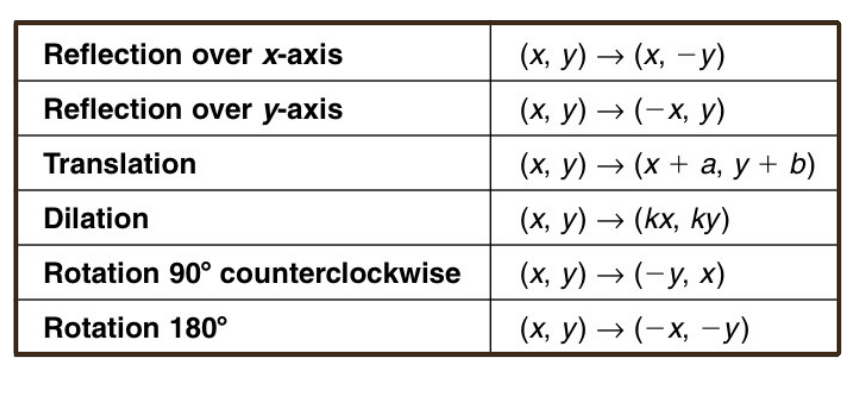
\includegraphics[width=0.8\textwidth]{transformation_r.png}
    \caption{A table of different transforms on a function}
    \label{fig:transformation_r}
\end{figure}

\section{Order is important!}

We can combine these transformations. This allows us, for example, to
translate a function up 2, then scale along the $y$ axis by 3.

Here is $y = 2.0 (\sin(x) + 1)$:
\begin{figure}[htbp]
    \centering

\begin{tikzpicture}[
tl/.style = {% tick labels
    fill=white, inner sep=1pt, font=\scriptsize,
            },                        ]
% grid
\draw[sdkblue, very thin, xstep=0.5236, ystep=0.5] (-6.6,-1.2) grid (6.6,4.2);

% y tick label
\foreach \y in {-1, -1/2, 1/2, 1, 2, 3, 4}{\node[tl,left=1mm] at (0,\y) {$\y$};}
% x tick label
\foreach \x [count=\xx from -4] in 
       {-2\pi,
        -\frac{3\pi}{2},
        -\pi,           
        -\frac{\pi}{2}, 
        { },
         \frac{\pi}{2},
         \pi, 
         \frac{3\pi}{2}, 
         2\pi
        }{\node[tl,below=1mm] at (3*0.5235*\xx,0) {$\x$};}
% axes
    \draw[->,thick] (-6.5,0) -- (6.5,0) node[right] {$x$};
    \draw[->,thick] (0,-1.25) -- (0, 4.25) node[above] {$y$};
% curve
\draw[<->,dashed,draw=black,
      domain=-6.5:6.5,samples=300,variable=\x] 
      plot (\x,{sin(deg{\x})});
\draw[<->,thick,draw=black,
      domain=-6.5:6.5,samples=300,variable=\x] 
      plot (\x,{2.0 * (sin(deg{\x}) + 1)});
\end{tikzpicture}

    \caption{A graph of the base function $\sin(x)$ and the transformed function $2(\sin(x)+1)$}
    \label{fig:translatingSin}
\end{figure}

A function is often a series of steps. Here are the steps in $f(x) = 2(\sin(x) + 1)$:
\begin{enumerate}
\item Take the sine of $x$
\item Add 1 to that
\item Multiply that by 2
\end{enumerate}
Note that this function can be distributed into $f(x) = 2\sin(x) + 2$ by bringing the 2 in both of the steps.

What if we change the order? Here are the steps in $g(x) = 2\sin(x) + 1$:
\begin{enumerate}
\item Take the sine of $x$
\item Multiply that by 2
\item Add 1 to that
\end{enumerate}
\begin{figure}[htbp]
    \centering

\begin{tikzpicture}[
tl/.style = {% tick labels
    fill=white, inner sep=1pt, font=\scriptsize,
            },                        ]
% grid
\draw[sdkblue, very thin, xstep=0.5236, ystep=0.5] (-6.6,-2.2) grid (6.6,4.2);

% y tick label
\foreach \y in {-2, -1, -1/2, 1/2, 1, 2, 3, 4}{\node[tl,left=1mm] at (0,\y) {$\y$};}
% x tick label
\foreach \x [count=\xx from -4] in 
       {-2\pi,
        -\frac{3\pi}{2},
        -\pi,           
        -\frac{\pi}{2}, 
        { },
         \frac{\pi}{2},
         \pi, 
         \frac{3\pi}{2}, 
         2\pi
        }{\node[tl,below=1mm] at (3*0.5235*\xx,0) {$\x$};}
% axes
    \draw[->,thick] (-6.5,0) -- (6.5,0) node[right] {$x$};
    \draw[->,thick] (0,-2.25) -- (0, 4.25) node[above] {$y$};
% curve
\draw[<->,dashed,draw=black,
      domain=-6.5:6.5,samples=300,variable=\x] 
plot (\x,{2.0 * (sin(deg{\x}) + 1)});
\draw (4, 3) node{$2(\sin(x) + 1)$};
\draw[<->,thick,draw=black,
      domain=-6.5:6.5,samples=300,variable=\x] 
      plot (\x,{2.0 * sin(deg(\x)) + 1});
\draw (2.5, -1.5) node{$2\sin(x) + 1$};
\end{tikzpicture}

    \caption{The functions $2\sin(x)+1$ in solid compared to $2(\sin(x)+1)$ in dashes.}
    \label{fig:orderMattersSin}
\end{figure}


The moral: You can do multiple transformations of your function, but
the order in which you do them is important.

\begin{Exercise}[title={Transforms}, label=sine_transform]

Find a function that creates a sine wave such that the top of the first crest is
at the point $(\frac{\pi}{2}, 5)$ and the bottom of the trough that follows is at $(\pi, 1)$.


\begin{tikzpicture}[
tl/.style = {% tick labels
    fill=white, inner sep=1pt, font=\scriptsize,
            },                        ]
% grid
\draw[sdkblue, very thin, xstep=0.5236, ystep=0.5] (-1,-0.6) grid (6.6,5.2);

% y tick label
\foreach \y in {1/2, 1, 2, 3, 4, 5}{\node[tl,left=1mm] at (0,\y) {$\y$};}
% axes
    \draw[->,thick] (-0.9,0) -- (6.5,0) node[right] {$x$};
    \draw[->,thick] (0,-0.25) -- (0, 5.25) node[above] {$y$};
    % curve
    \filldraw[black] (1.570796326794897, 5)  circle(3pt) node [right, yshift=1mm]{$(\pi/2,5)$};
    \filldraw[black] (3.141592653589793, 1)  circle(3pt) node[below]{$(\pi,1)$};
    \draw[<->,thick,draw=black,
      domain=-0.5:6.5,samples=300,variable=\x] 
      plot (\x,{2.0 * sin(deg{2*\x} - 90) + 3});
\end{tikzpicture}

  
\end{Exercise}
\begin{Answer}[ref=sine_transform]

\begin{tikzpicture}[
tl/.style = {% tick labels
    fill=white, inner sep=1pt, font=\scriptsize,
            },                        ]
% grid
\draw[sdkblue, very thin, xstep=0.5236, ystep=0.5] (-1,-0.6) grid (6.6,5.2);

% y tick label
\foreach \y in {1/2, 1, 2, 3, 4, 5}{\node[tl,left=1mm] at (0,\y) {$\y$};}
% axes
    \draw[->,thick] (-0.9,0) -- (6.5,0) node[right] {$x$};
    \draw[->,thick] (0,-0.25) -- (0, 5.25) node[above] {$y$};
    % curvet
    \filldraw[black] (0.785398163397448, 3)  circle(3pt) node[right, yshift=1mm]{$(\pi/4, 3)$};
    \filldraw[black] (1.570796326794897, 5)  circle(3pt) node [right, yshift=1mm]{$(\pi/2, 5)$};
    \filldraw[black] (3.141592653589793, 1)  circle(3pt) node[below]{$(\pi, 1)$};
    \filldraw[black] (4.71238898038469, 5)  circle(3pt) node[right, yshift=1mm]{$(3\pi/2, 5)$};
    \draw[<->,thick,draw=black,
      domain=-0.5:6.5,samples=300,variable=\x] 
      plot (\x,{2.0 * sin(deg{2*\x} - 90) + 3});
    \draw[dashed,thick, draw=black] (0,3) -- (6,3);
\end{tikzpicture}

This wave has an amplitude of 2; its baseline has been translated up to 3.

This wave has wavelength of $\pi$. A sine wave usually has a
wavelength of $2\pi$, so we need to compress the $x$ axis by a factor of 2.

The wave first crosses its baseline at $pi/4$.  The sine wave starts
by crossing its baseline, so we need to translate the curve right by
$\pi/4$.

$$f(x) = 2 \sin(2x - \frac{\pi}{4}) + 3$$

\end{Answer}

\section{Effects on even and odd Functions}
Now that you've worked with transformations like shifts and scalings, you can use symmetry to quickly assess how those changes affect a function.
\begin{enumerate}
    \item Vertical shifts (like \( f(x) + c \)) do not change whether a function is even or odd — but they break symmetry about the origin or y-axis. Example: \( x^2 + 1 \) is still even, but it's not symmetric about the origin.
    \item Horizontal shifts (like \( f(x - c) \)) also typically destroy even/odd symmetry. Example: \( f(x) = \sin(x) \) is odd. But \( f(x) = \sin(x - \pi/2) \) is neither even nor odd.
    \item Vertical scalings (like \( a \cdot f(x) \)) preserve symmetry type. Example: \( x^2 \) versus \( 3x^2 \).
    \item Horizontal scalings (like \( f(bx) \)) preserve symmetry as long as the center of the transformation stays aligned. Example: \( f(x) = x^3 \) is odd. \( f(x) = (2x)^3 \) is still odd.
\end{enumerate}

Remember these key ideas:
\begin{enumerate}
    \item Reflecting an even function over the y-axis? It remains unchanged.
    \item Reflecting an odd function over the origin? Still unchanged.
    \item But any shift left or right often breaks the symmetry, so check \( f(-x) \) again if you've applied one.
\end{enumerate}

